\documentclass[11pt, a4paper]{article}

% Fonts and Encoding
\usepackage[utf8]{inputenc}
\usepackage[T1]{fontenc}

% Math and Symbols
\usepackage{amsmath, amssymb, amsthm, amsfonts, mathrsfs, mathtools}

% Layout and Geometry
\usepackage{geometry}
\geometry{a4paper, margin=1in}

% Formatting and Graphics
\usepackage{graphicx, xcolor, enumitem, booktabs, array, tabularx}

% TikZ for Illustrations
\usepackage{tikz}
\usetikzlibrary{arrows.meta, positioning, shapes.geometric, calc, backgrounds, matrix}

% Clickable Links and TOC
\usepackage{hyperref}
\hypersetup{
    colorlinks=true,
    linkcolor=blue,
    filecolor=magenta,      
    urlcolor=cyan,
    pdftitle={Advanced Probability Theory: The Gamma Distribution},
}

% Theorem Environments
\newtheorem{theorem}{Theorem}[section]
\newtheorem{lemma}[theorem]{Lemma}
\newtheorem{proposition}[theorem]{Proposition}
\newtheorem{corollary}[theorem]{Corollary}
\theoremstyle{definition}
\newtheorem{definition}{Definition}[section]
\newtheorem{axiom}{Axiom}[section]
\newtheorem{example}{Example}[section]
\theoremstyle{remark}
\newtheorem{remark}{Remark}[section]

% Custom Commands (Enforced standard notation)
\newcommand{\R}{\mathbb{R}}
\newcommand{\N}{\mathbb{N}}
\newcommand{\Z}{\mathbb{Z}}
\newcommand{\Q}{\mathbb{Q}}
\newcommand{\E}{\mathbb{E}}
\newcommand{\Prob}{\mathbb{P}}
\newcommand{\F}{\mathcal{F}}

\begin{document}

\title{\textbf{Advanced Probability Theory: The Gamma Distribution and its Applications \\ \large A Rigorous Mathematical and Quantitative Modeling Approach}}
\author{Tashfeen Omran}
\date{\today}

\maketitle
\tableofcontents
\newpage

\section{Concept Checklist \& Question Mapping}

The following table maps the core theoretical concepts, logical structures, and proof techniques extracted from the foundational text to the corresponding problems in this document.

\vspace{1em}
\noindent
\renewcommand{\arraystretch}{1.5}
\begin{tabularx}{\textwidth}{l X l}
\toprule
\textbf{Code} & \textbf{Concept / Proof Technique} & \textbf{Problem Mapping} \\
\midrule
\textbf{C1} & Gamma Function Properties \& Analytic Proofs (Integration by parts, limits) & 1, 2, 3, 5 \\
\textbf{C2} & Gamma Density Normalization \& The ``Kernel Trick'' & 4, 16, 17 \\
\textbf{C3} & Exponential Distribution \& Memoryless Property (Proofs \& Counterexamples) & 6, 7, 8, 9, 10 \\
\textbf{C4} & Chi-Square Distribution, Degrees of Freedom, \& Transformations & 11, 12, 14, 15 \\
\textbf{C5} & Generalized Moments \& Non-Linear Expectations (LOTUS, existence) & 16, 17, 18, 19, 20 \\
\textbf{C6} & Distributional Transformations \& Jacobians (Continuous to Discrete/Continuous) & 13, 21, 22, 23 \\
\textbf{C7} & Moment Generating Functions (MGF) \& Sums of Independent Variables & 12, 24 \\
\textbf{C8} & Bayesian Inference \& Conjugate Priors (Poisson-Gamma model) & 26 \\
\textbf{C9} & Abstract Real-World Modeling (Jump-Diffusion, Algorithmic Finance) & 27, 30 \\
\textbf{C10} & Diagnostic Testing \& Fallacy Identification (Finding flaws in logic) & 8, 14, 18, 25 \\
\textbf{C11} & Set-Theoretic Probability \& Asymptotic Bounds (Borel-Cantelli, Hazard Rates) & 28, 29 \\
\bottomrule
\end{tabularx}
\vspace{1em}

\newpage

\section{Advanced Practice Problem Set}

\subsection{Foundations \& The Gamma Function}
\begin{enumerate}[label=\textbf{\arabic*.}]
    \item \textbf{Prove that} $\Gamma(1/2) = \sqrt{\pi}$ by utilizing the standard Gaussian integral $\int_{-\infty}^{\infty} e^{-x^2} dx = \sqrt{\pi}$.
    \item \textbf{Prove that} for any real $\alpha > 0$, $\Gamma(\alpha + 1) = \alpha \Gamma(\alpha)$ using rigorous integration by parts, explicitly demonstrating the evaluation of boundary limits.
    \item \textbf{Derive} the mode of the Gamma distribution for $\alpha > 1$. Furthermore, \textbf{prove} that for $\alpha \le 1$, the density function is strictly decreasing on $(0, \infty)$ and thus possesses no interior mode.
    \item \textbf{Prove} the ``Kernel Trick'' identity: For any $\alpha > 0, \beta > 0$, show that $\int_{0}^{\infty} y^{\alpha-1} e^{-y/\beta} dy = \beta^\alpha \Gamma(\alpha)$ without using integration by parts.
    \item \textbf{Find a counterexample to} the claim that the Gamma function $\Gamma(x)$ is strictly monotonically increasing for all $x > 0$.
\end{enumerate}

\subsection{The Exponential Distribution \& Memoryless Properties}
\begin{enumerate}[label=\textbf{\arabic*.}, resume]
    \item \textbf{Prove that} if $Y \sim \text{Exp}(\beta)$, it satisfies the memoryless property: $\Prob(Y > a + b \mid Y > a) = \Prob(Y > b)$ for all $a, b > 0$.
    \item \textbf{Establish the logical equivalence} between the continuous memoryless property and the Exponential distribution. Specifically, prove that if a continuous, strictly positive random variable $Y$ satisfies $\Prob(Y > a + b) = \Prob(Y > a)\Prob(Y > b)$, then $Y$ must be Exponentially distributed.
    \item \textbf{Find a counterexample to} the memoryless property for a general Gamma distribution by evaluating $\Prob(Y > 2 \mid Y > 1)$ for $Y \sim \text{Gamma}(2, 1)$ and showing it does not equal $\Prob(Y > 1)$.
    \item \textbf{Derive the probability measure for} $M = \min(Y_1, Y_2, \dots, Y_n)$, where $Y_i \sim \text{Exp}(\beta)$ are independent and identically distributed.
    \item \textbf{Establish the logical equivalence of} a Poisson process and Exponential waiting times: If the number of events in time $t$, $N(t)$, follows a Poisson distribution with rate $\lambda t$, prove that the time until the first event $T_1$ follows an Exponential distribution with mean $1/\lambda$.
\end{enumerate}

\subsection{Chi-Square Distributions \& Transformations}
\begin{enumerate}[label=\textbf{\arabic*.}, resume]
    \item \textbf{Derive the probability density function for} $Y = X^2$, where $X \sim \mathcal{N}(0,1)$. Prove that $Y \sim \chi^2_1$ by matching it to the Gamma distribution parameters.
    \item \textbf{Prove that} the sum of $n$ independent $\chi^2_1$ random variables follows a $\chi^2_n$ distribution by deriving and utilizing the Moment Generating Function (MGF).
    \item \textbf{Derive the probability measure for} $W = \sqrt{Y}$, where $Y \sim \text{Gamma}(\alpha, \beta)$. (This generalizes the Rayleigh and Nakagami distributions).
    \item \textbf{Find the flaw in the following statement:} ``Let $X \sim \chi^2_5$ and $Y \sim \chi^2_3$ be independent. Since variances add, the distribution of $Z = X - Y$ is $\chi^2_2$.'' Provide the rigorous mathematical correction.
    \item \textbf{Derive} the expected value $\E[1/Y]$ for $Y \sim \chi^2_\nu$. State and prove the strict condition on the degrees of freedom $\nu$ required for this inverse moment to exist.
\end{enumerate}

\subsection{Generalized Moments \& Non-Linear Expectations}
\begin{enumerate}[label=\textbf{\arabic*.}, resume]
    \item \textbf{Prove} the generalized moment formula for a Gamma random variable $Y \sim \text{Gamma}(\alpha, \beta)$: $\E[Y^a] = \frac{\beta^a \Gamma(\alpha + a)}{\Gamma(\alpha)}$, explicitly stating the domain of $a$ for which this expectation is finite.
    \item \textbf{Derive} the variance of $Y^2$, denoted as $\text{Var}(Y^2)$, for $Y \sim \text{Gamma}(\alpha, \beta)$ using the generalized moment formula.
    \item \textbf{Find a counterexample to} the existence of the second inverse moment $\E[Y^{-2}]$ for an Exponential distribution ($\alpha = 1$). Prove rigorously that the integral diverges.
    \item \textbf{Derive} the skewness of the Gamma distribution, defined as $\E[(Y - \mu)^3] / \sigma^3$. Prove that as $\alpha \to \infty$, the skewness approaches $0$.
    \item \textbf{Derive} the excess kurtosis of the Gamma distribution, defined as $(\E[(Y - \mu)^4] / \sigma^4) - 3$.
\end{enumerate}

\subsection{Advanced Transformations \& Discretization}
\begin{enumerate}[label=\textbf{\arabic*.}, resume]
    \item \textbf{Prove that} if $Y \sim \text{Exp}(\beta)$, the discretized random variable $X = \lfloor Y \rfloor$ (the floor of $Y$) follows a Geometric distribution. Determine its success probability $p$.
    \item \textbf{Derive the probability density function of} $X = \frac{Y_1}{Y_1 + Y_2}$, where $Y_1 \sim \text{Gamma}(\alpha_1, \beta)$ and $Y_2 \sim \text{Gamma}(\alpha_2, \beta)$ are independent. Prove that $X$ follows a Beta distribution.
    \item \textbf{Prove} the scaling property of the Gamma distribution: If $Y \sim \text{Gamma}(\alpha, \beta)$ and $c > 0$ is a constant, then $cY \sim \text{Gamma}(\alpha, c\beta)$ using the cumulative distribution function (CDF) method.
    \item \textbf{Establish the logical equivalence of} the Moment Generating Function $M_Y(t) = (1 - \beta t)^{-\alpha}$ and the Taylor series expansion of moments $\sum_{k=0}^{\infty} \frac{t^k}{k!} \E[Y^k]$. Prove they yield the same formula for $\E[Y^2]$.
    \item \textbf{Find the flaw in the following proof:} ``Let $Y \sim \text{Gamma}(\alpha, \beta)$. By the linearity of the natural logarithm, $\E[\ln Y] = \ln(\E[Y]) = \ln(\alpha\beta)$.'' Use Jensen's Inequality to prove the correct relationship.
\end{enumerate}

\subsection{Abstract Applications: Bayesian Inference \& Finance}
\begin{enumerate}[label=\textbf{\arabic*.}, resume]
    \item \textbf{Derive the posterior predictive distribution} for a new observation $x_{new}$ in a Bayesian model where the data $X \mid \lambda \sim \text{Poisson}(\lambda)$ and the prior is $\lambda \sim \text{Gamma}(\alpha, \beta)$. Prove that the marginal distribution of $X$ is Negative Binomial.
    \item \textbf{Model Problem Setup (Jump-Diffusion):} In quantitative finance, market crashes occur according to a Poisson process with rate $\lambda$. The time until the $n$-th crash is $Y \sim \text{Gamma}(n, 1/\lambda)$. Derive the exact probability that the $n$-th crash occurs before time $T$.
    \item \textbf{Prove that} the hazard rate function $h(y) = \frac{f(y)}{1 - F(y)}$ of a Gamma distribution is strictly monotonically increasing if $\alpha > 1$, and strictly monotonically decreasing if $\alpha < 1$.
    \item \textbf{Set-Theoretic Probability:} Let $Y \sim \text{Exp}(\beta)$. Define the sequence of events $A_n = \{Y > n\}$. Using the Borel-Cantelli Lemma, prove that $\Prob(\limsup_{n \to \infty} A_n) = 0$.
    \item \textbf{Algorithmic Finance Optimization:} A trading algorithm incurs a holding cost $c_1$ if a transaction time $Y \sim \text{Exp}(\beta)$ exceeds a threshold $t$, and a deterministic execution cost $c_2 t$. Derive the optimal threshold $t^*$ that minimizes the expected cost function $C(t) = c_1 \Prob(Y > t) + c_2 t$.
\end{enumerate}

\newpage

\section{Detailed Rigorous Solutions}

\begin{proof}[Solution to Problem 1]
We are given the definition of the Gamma function: $\Gamma(\alpha) = \int_0^\infty y^{\alpha-1} e^{-y} dy$. We wish to evaluate $\Gamma(1/2)$.
\[ \Gamma(1/2) = \int_0^\infty y^{-1/2} e^{-y} dy \]
We apply the substitution $y = x^2$. The differential is $dy = 2x \, dx$. The limits of integration remain $0$ to $\infty$.
\begin{align*}
\Gamma(1/2) &= \int_0^\infty (x^2)^{-1/2} e^{-x^2} (2x \, dx) \\
&= \int_0^\infty x^{-1} e^{-x^2} 2x \, dx \\
&= 2 \int_0^\infty e^{-x^2} dx
\end{align*}
Since the integrand $e^{-x^2}$ is an even function, the integral from $0$ to $\infty$ is exactly half of the integral from $-\infty$ to $\infty$.
\[ \Gamma(1/2) = 2 \left( \frac{1}{2} \int_{-\infty}^\infty e^{-x^2} dx \right) = \int_{-\infty}^\infty e^{-x^2} dx \]
By the standard Gaussian integral, $\int_{-\infty}^\infty e^{-x^2} dx = \sqrt{\pi}$. Therefore, $\Gamma(1/2) = \sqrt{\pi}$.
\end{proof}

\begin{proof}[Solution to Problem 2]
By definition, $\Gamma(\alpha + 1) = \int_0^\infty y^{(\alpha+1)-1} e^{-y} dy = \int_0^\infty y^\alpha e^{-y} dy$.
We proceed using integration by parts: $\int u \, dv = uv - \int v \, du$.
Let $u = y^\alpha$ and $dv = e^{-y} dy$.
Then $du = \alpha y^{\alpha-1} dy$ and $v = -e^{-y}$.
\begin{align*}
\Gamma(\alpha + 1) &= \lim_{b \to \infty} \left[ -y^\alpha e^{-y} \right]_0^b - \int_0^\infty (-e^{-y}) \alpha y^{\alpha-1} dy \\
&= \lim_{b \to \infty} \left( \frac{-b^\alpha}{e^b} \right) - \left( -0^\alpha e^{-0} \right) + \alpha \int_0^\infty y^{\alpha-1} e^{-y} dy
\end{align*}
Since $\alpha > 0$, $0^\alpha = 0$. For the upper limit, exponential growth dominates polynomial growth. Applying L'H\^{o}pital's rule $\lceil \alpha \rceil$ times yields:
\[ \lim_{b \to \infty} \frac{b^\alpha}{e^b} = 0 \]
Thus, the boundary terms vanish completely.
\[ \Gamma(\alpha + 1) = 0 - 0 + \alpha \int_0^\infty y^{\alpha-1} e^{-y} dy = \alpha \Gamma(\alpha) \]
\end{proof}

\begin{proof}[Solution to Problem 3]
Let $f(y) = \frac{1}{\beta^\alpha \Gamma(\alpha)} y^{\alpha-1} e^{-y/\beta}$ for $y > 0$. To find the mode, we maximize $f(y)$ by finding the critical points of its natural logarithm, $\ln f(y)$, which is strictly monotonic and preserves extrema.
\[ \ln f(y) = -\ln(\beta^\alpha \Gamma(\alpha)) + (\alpha - 1)\ln y - \frac{y}{\beta} \]
Taking the derivative with respect to $y$:
\[ \frac{d}{dy} \ln f(y) = \frac{\alpha - 1}{y} - \frac{1}{\beta} \]
Setting the derivative to zero to find the critical point $y^*$:
\[ \frac{\alpha - 1}{y^*} = \frac{1}{\beta} \implies y^* = \beta(\alpha - 1) \]
For $\alpha > 1$, $y^* > 0$, which is in the support of the distribution. The second derivative is $-\frac{\alpha-1}{y^2} < 0$, confirming a global maximum. Thus, the mode is $\beta(\alpha - 1)$.

If $\alpha \le 1$, then $\alpha - 1 \le 0$. Since $y > 0$ and $\beta > 0$, the derivative $\frac{d}{dy} \ln f(y) = \frac{\alpha - 1}{y} - \frac{1}{\beta}$ is strictly negative for all $y > 0$. Therefore, $f(y)$ is strictly decreasing on $(0, \infty)$ and the supremum occurs as $y \to 0^+$. No interior mode exists.

\vspace{1em}
\begin{center}
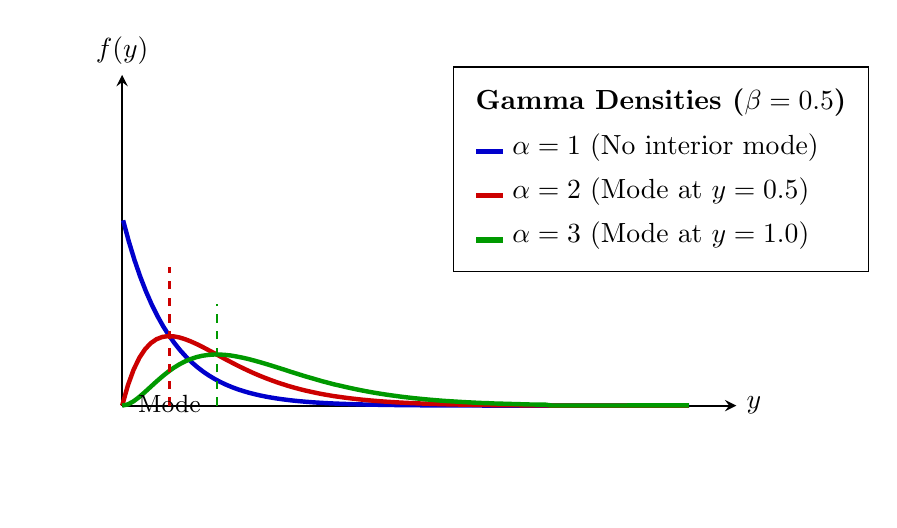
\begin{tikzpicture}[scale=1.2]
\fill[white] (-1,-1) rectangle (7,4);
\draw[thick, ->, >=stealth] (0,0) -- (6.5,0) node[right] {$y$};
\draw[thick, ->, >=stealth] (0,0) -- (0,3.5) node[above] {$f(y)$};

% alpha = 1 (Exponential, strictly decreasing)
\draw[ultra thick, blue!80!black, domain=0.01:6, samples=100] plot (\x, {2*exp(-2*\x)});
% alpha = 2 (Mode at beta(2-1) = 0.5)
\draw[ultra thick, red!80!black, domain=0:6, samples=100] plot (\x, {4*\x*exp(-2*\x)});
% alpha = 3 (Mode at beta(3-1) = 1.0)
\draw[ultra thick, green!60!black, domain=0:6, samples=100] plot (\x, {4*\x*\x*exp(-2*\x)});

% Mode indicators
\draw[thick, dashed, red!80!black] (0.5, 0) -- (0.5, 1.47) node[below=1.5cm, black] {\small Mode};
\draw[thick, dashed, green!60!black] (1, 0) -- (1, 1.08);

\node[align=left, anchor=west, inner sep=8pt, draw=black, fill=white] at (3.5, 2.5) {
    \textbf{Gamma Densities ($\beta=0.5$)} \\[4pt]
    \textcolor{blue!80!black}{\rule{10pt}{2pt}} $\alpha=1$ (No interior mode) \\[4pt]
    \textcolor{red!80!black}{\rule{10pt}{2pt}} $\alpha=2$ (Mode at $y=0.5$) \\[4pt]
    \textcolor{green!60!black}{\rule{10pt}{2pt}} $\alpha=3$ (Mode at $y=1.0$)
};
\end{tikzpicture}
\end{center}
\end{proof}

\begin{proof}[Solution to Problem 4]
We wish to evaluate $I = \int_{0}^{\infty} y^{\alpha-1} e^{-y/\beta} dy$.
We use the substitution $u = y/\beta$. Since $\beta > 0$, as $y \to 0, u \to 0$ and as $y \to \infty, u \to \infty$.
The differential is $dy = \beta \, du$, and $y = \beta u$.
\begin{align*}
I &= \int_{0}^{\infty} (\beta u)^{\alpha-1} e^{-u} (\beta \, du) \\
&= \int_{0}^{\infty} \beta^{\alpha-1} u^{\alpha-1} e^{-u} \beta \, du \\
&= \beta^\alpha \int_{0}^{\infty} u^{\alpha-1} e^{-u} du
\end{align*}
By Definition 1.1 of the Gamma function, the remaining integral is exactly $\Gamma(\alpha)$.
Thus, $I = \beta^\alpha \Gamma(\alpha)$. This ``Kernel Trick'' proves that the normalizing constant required to make the Gamma PDF integrate to 1 is exactly $\frac{1}{\beta^\alpha \Gamma(\alpha)}$.
\end{proof}

\begin{proof}[Solution to Problem 5]
To disprove the claim that $\Gamma(x)$ is strictly monotonically increasing for all $x > 0$, we only need to find two points $x_1 < x_2$ such that $\Gamma(x_1) \ge \Gamma(x_2)$.
Consider $x_1 = 1$ and $x_2 = 2$.
By definition, $\Gamma(1) = \int_0^\infty e^{-y} dy = 1$.
Using the recursive property $\Gamma(n) = (n-1)!$ for integers, $\Gamma(2) = (2-1)! = 1! = 1$.
Since $1 < 2$ but $\Gamma(1) = \Gamma(2) = 1$, the function is not strictly monotonically increasing. In fact, $\Gamma(x)$ has a global minimum on the positive real axis at approximately $x \approx 1.4616$.
\end{proof}

\begin{proof}[Solution to Problem 6]
Let $Y \sim \text{Exp}(\beta)$. The cumulative distribution function is $F(y) = 1 - e^{-y/\beta}$ for $y > 0$. The survival function is $\Prob(Y > y) = 1 - F(y) = e^{-y/\beta}$.
We evaluate the conditional probability $\Prob(Y > a + b \mid Y > a)$ using the definition of conditional probability $\Prob(A \mid B) = \frac{\Prob(A \cap B)}{\Prob(B)}$.
Since $a, b > 0$, the event $\{Y > a + b\}$ is a subset of $\{Y > a\}$. Thus, their intersection is simply $\{Y > a + b\}$.
\begin{align*}
\Prob(Y > a + b \mid Y > a) &= \frac{\Prob(Y > a + b)}{\Prob(Y > a)} \\
&= \frac{e^{-(a+b)/\beta}}{e^{-a/\beta}} \\
&= e^{-(a+b)/\beta - (-a/\beta)} \\
&= e^{-b/\beta}
\end{align*}
Since $e^{-b/\beta} = \Prob(Y > b)$, we have proven $\Prob(Y > a + b \mid Y > a) = \Prob(Y > b)$.
\end{proof}

\begin{proof}[Solution to Problem 7]
Let $g(y) = \Prob(Y > y)$. The memoryless property states $\Prob(Y > a + b \mid Y > a) = \Prob(Y > b)$, which implies:
\[ \frac{\Prob(Y > a + b)}{\Prob(Y > a)} = \Prob(Y > b) \implies g(a+b) = g(a)g(b) \]
This is Cauchy's functional equation. Since $Y$ is a continuous random variable, its survival function $g(y)$ is right-continuous and monotonically decreasing.
The only non-trivial solutions to $g(a+b) = g(a)g(b)$ under the condition of monotonicity and $g(0)=1$ are of the form $g(y) = e^{-cy}$ for some constant $c > 0$.
Let $c = 1/\beta$. Then $g(y) = \Prob(Y > y) = e^{-y/\beta}$.
The cumulative distribution function is $F(y) = 1 - g(y) = 1 - e^{-y/\beta}$. Taking the derivative yields the PDF $f(y) = \frac{1}{\beta} e^{-y/\beta}$, which is exactly the Exponential distribution. Thus, logical equivalence is established.
\end{proof}

\begin{proof}[Solution to Problem 8]
Let $Y \sim \text{Gamma}(2, 1)$. The PDF is $f(y) = \frac{1}{1^2 \Gamma(2)} y^{2-1} e^{-y/1} = y e^{-y}$.
We calculate $\Prob(Y > y)$ using integration by parts:
\[ \Prob(Y > y) = \int_y^\infty x e^{-x} dx = \left[ -x e^{-x} \right]_y^\infty - \int_y^\infty (-e^{-x}) dx = y e^{-y} + e^{-y} = (y+1)e^{-y} \]
Now we test the memoryless property for $a=1, b=1$.
$\Prob(Y > 1) = (1+1)e^{-1} = 2e^{-1}$.
$\Prob(Y > 2) = (2+1)e^{-2} = 3e^{-2}$.
The conditional probability is:
\[ \Prob(Y > 2 \mid Y > 1) = \frac{\Prob(Y > 2)}{\Prob(Y > 1)} = \frac{3e^{-2}}{2e^{-1}} = 1.5 e^{-1} \]
However, $\Prob(Y > 1) = 2e^{-1}$. Since $1.5 e^{-1} \neq 2e^{-1}$, the memoryless property fails for $\alpha = 2$.
\end{proof}

\begin{proof}[Solution to Problem 9]
Let $M = \min(Y_1, Y_2, \dots, Y_n)$ where $Y_i \sim \text{Exp}(\beta)$ are i.i.d.
The event $\{M > m\}$ occurs if and only if every individual $Y_i > m$.
\[ \Prob(M > m) = \Prob(Y_1 > m \cap Y_2 > m \cap \dots \cap Y_n > m) \]
By independence, the joint probability factors into the product of marginal probabilities:
\[ \Prob(M > m) = \prod_{i=1}^n \Prob(Y_i > m) \]
For an Exponential distribution, $\Prob(Y_i > m) = e^{-m/\beta}$.
\[ \Prob(M > m) = \prod_{i=1}^n e^{-m/\beta} = \left( e^{-m/\beta} \right)^n = e^{-nm/\beta} \]
The CDF of $M$ is $F_M(m) = 1 - \Prob(M > m) = 1 - e^{-m/(\beta/n)}$.
This is the CDF of an Exponential distribution with scale parameter $\beta/n$. Thus, $M \sim \text{Exp}(\beta/n)$.
\end{proof}

\begin{proof}[Solution to Problem 10]
Let $N(t)$ be the number of events in time interval $[0, t]$, where $N(t) \sim \text{Poisson}(\lambda t)$. The probability mass function is $\Prob(N(t) = k) = \frac{(\lambda t)^k e^{-\lambda t}}{k!}$.
Let $T_1$ be the continuous random variable representing the time until the first event.
The event $\{T_1 > t\}$ means that strictly zero events have occurred in the interval $[0, t]$.
Therefore, the events are logically equivalent: $\{T_1 > t\} \iff \{N(t) = 0\}$.
We compute the probability:
\[ \Prob(T_1 > t) = \Prob(N(t) = 0) = \frac{(\lambda t)^0 e^{-\lambda t}}{0!} = e^{-\lambda t} \]
The cumulative distribution function for $T_1$ is $F(t) = 1 - \Prob(T_1 > t) = 1 - e^{-\lambda t}$.
This is the exact CDF of an Exponential distribution with scale parameter $\beta = 1/\lambda$.
\end{proof}

\begin{proof}[Solution to Problem 11]
Let $X \sim \mathcal{N}(0,1)$. The PDF of $X$ is $f_X(x) = \frac{1}{\sqrt{2\pi}} e^{-x^2/2}$.
Let $Y = X^2$. We find the CDF of $Y$, $F_Y(y) = \Prob(Y \le y)$. Since $Y \ge 0$, $F_Y(y) = 0$ for $y < 0$. For $y \ge 0$:
\[ F_Y(y) = \Prob(X^2 \le y) = \Prob(-\sqrt{y} \le X \le \sqrt{y}) = F_X(\sqrt{y}) - F_X(-\sqrt{y}) \]
Differentiating with respect to $y$ to find the PDF $f_Y(y)$:
\[ f_Y(y) = \frac{d}{dy} \left[ F_X(\sqrt{y}) - F_X(-\sqrt{y}) \right] = f_X(\sqrt{y}) \cdot \frac{1}{2\sqrt{y}} - f_X(-\sqrt{y}) \cdot \left( -\frac{1}{2\sqrt{y}} \right) \]
Since the standard normal PDF is symmetric, $f_X(\sqrt{y}) = f_X(-\sqrt{y})$.
\[ f_Y(y) = 2 f_X(\sqrt{y}) \frac{1}{2\sqrt{y}} = \frac{1}{\sqrt{y}} \frac{1}{\sqrt{2\pi}} e^{-(\sqrt{y})^2/2} = \frac{1}{\sqrt{2\pi}} y^{-1/2} e^{-y/2} \]
We know $\Gamma(1/2) = \sqrt{\pi}$, so $\sqrt{2\pi} = \sqrt{2}\Gamma(1/2) = 2^{1/2}\Gamma(1/2)$.
\[ f_Y(y) = \frac{1}{2^{1/2}\Gamma(1/2)} y^{(1/2)-1} e^{-y/2} \]
This perfectly matches the Gamma PDF $f(y) = \frac{1}{\beta^\alpha \Gamma(\alpha)} y^{\alpha-1} e^{-y/\beta}$ with $\alpha = 1/2$ and $\beta = 2$. By definition, Gamma$(1/2, 2)$ is the $\chi^2_1$ distribution.
\end{proof}

\begin{proof}[Solution to Problem 12]
Let $Y_i \sim \chi^2_1$ for $i = 1, \dots, n$ be independent. A $\chi^2_1$ distribution is equivalent to Gamma$(1/2, 2)$.
The MGF of a Gamma$(\alpha, \beta)$ distribution is $M(t) = (1 - \beta t)^{-\alpha}$.
Thus, the MGF of each $Y_i$ is $M_{Y_i}(t) = (1 - 2t)^{-1/2}$.
Let $W = \sum_{i=1}^n Y_i$. Because the variables are independent, the MGF of their sum is the product of their individual MGFs:
\[ M_W(t) = \prod_{i=1}^n M_{Y_i}(t) = \prod_{i=1}^n (1 - 2t)^{-1/2} = \left( (1 - 2t)^{-1/2} \right)^n = (1 - 2t)^{-n/2} \]
We recognize $(1 - 2t)^{-n/2}$ as the MGF of a Gamma distribution with $\alpha = n/2$ and $\beta = 2$. By definition, Gamma$(n/2, 2)$ is the $\chi^2_n$ distribution. Therefore, $W \sim \chi^2_n$.
\end{proof}

\begin{proof}[Solution to Problem 13]
Let $Y \sim \text{Gamma}(\alpha, \beta)$ with PDF $f_Y(y) = \frac{1}{\beta^\alpha \Gamma(\alpha)} y^{\alpha-1} e^{-y/\beta}$ for $y > 0$.
Let $W = \sqrt{Y}$. The transformation is strictly increasing for $y > 0$. The inverse transformation is $y = w^2$.
The Jacobian of the transformation is $\left| \frac{dy}{dw} \right| = \left| 2w \right| = 2w$ (since $w > 0$).
By the transformation method, $f_W(w) = f_Y(w^2) \left| \frac{dy}{dw} \right|$.
\begin{align*}
f_W(w) &= \frac{1}{\beta^\alpha \Gamma(\alpha)} (w^2)^{\alpha-1} e^{-w^2/\beta} (2w) \\
&= \frac{2}{\beta^\alpha \Gamma(\alpha)} w^{2\alpha-2} w^1 e^{-w^2/\beta} \\
&= \frac{2}{\beta^\alpha \Gamma(\alpha)} w^{2\alpha-1} e^{-w^2/\beta}, \quad w > 0
\end{align*}
This is the generalized Rayleigh (or Nakagami) distribution probability measure.
\end{proof}

\begin{proof}[Solution to Problem 14]
The flaw lies in the statement ``Since variances add, the distribution of $Z = X - Y$ is $\chi^2_2$.''
While it is true that for independent random variables $\text{Var}(X - Y) = \text{Var}(X) + \text{Var}(Y)$, the \textit{distribution} of a difference of independent Gamma (or Chi-Square) variables is \textbf{not} Gamma.
A Chi-Square random variable is strictly non-negative (support is $[0, \infty)$). However, $Z = X - Y$ can take negative values because it is possible for $Y > X$. A distribution with support on the entire real line $(-\infty, \infty)$ cannot be a Chi-Square distribution. The MGF of $Z$ is $M_Z(t) = M_X(t)M_{-Y}(t) = (1-2t)^{-5/2}(1+2t)^{-3/2}$, which does not match the Chi-Square MGF form $(1-2t)^{-\nu/2}$.
\end{proof}

\begin{proof}[Solution to Problem 15]
Let $Y \sim \chi^2_\nu \equiv \text{Gamma}(\nu/2, 2)$. We want to find $\E[Y^{-1}]$.
By the Law of the Unconscious Statistician (LOTUS):
\[ \E[Y^{-1}] = \int_0^\infty y^{-1} \frac{1}{2^{\nu/2} \Gamma(\nu/2)} y^{(\nu/2)-1} e^{-y/2} dy = \frac{1}{2^{\nu/2} \Gamma(\nu/2)} \int_0^\infty y^{(\nu/2 - 1)-1} e^{-y/2} dy \]
The integral is the kernel of a Gamma distribution with parameters $\alpha_{new} = \nu/2 - 1$ and $\beta = 2$.
For the integral to converge (and thus for the Gamma function to be defined), we strictly require the new shape parameter to be positive: $\nu/2 - 1 > 0 \implies \nu > 2$.
Assuming $\nu > 2$, the integral evaluates to $2^{\nu/2 - 1} \Gamma(\nu/2 - 1)$ via the Kernel Trick.
\[ \E[Y^{-1}] = \frac{2^{\nu/2 - 1} \Gamma(\nu/2 - 1)}{2^{\nu/2} \Gamma(\nu/2)} = \frac{2^{-1} \Gamma(\nu/2 - 1)}{(\nu/2 - 1)\Gamma(\nu/2 - 1)} = \frac{1}{2(\nu/2 - 1)} = \frac{1}{\nu - 2} \]
\end{proof}

\begin{proof}[Solution to Problem 16]
Let $Y \sim \text{Gamma}(\alpha, \beta)$. We seek $\E[Y^a]$.
\[ \E[Y^a] = \int_0^\infty y^a \frac{1}{\beta^\alpha \Gamma(\alpha)} y^{\alpha-1} e^{-y/\beta} dy = \frac{1}{\beta^\alpha \Gamma(\alpha)} \int_0^\infty y^{(\alpha+a)-1} e^{-y/\beta} dy \]
The integral represents the unnormalized kernel of a Gamma distribution with shape parameter $\alpha + a$ and scale parameter $\beta$.
For this improper integral to converge at the lower bound $y \to 0$, we must have $\alpha + a > 0$.
If $\alpha + a > 0$, we apply the Kernel Trick (Problem 4): $\int_0^\infty y^{(\alpha+a)-1} e^{-y/\beta} dy = \beta^{\alpha+a} \Gamma(\alpha+a)$.
\[ \E[Y^a] = \frac{\beta^{\alpha+a} \Gamma(\alpha+a)}{\beta^\alpha \Gamma(\alpha)} = \frac{\beta^a \beta^\alpha \Gamma(\alpha+a)}{\beta^\alpha \Gamma(\alpha)} = \frac{\beta^a \Gamma(\alpha+a)}{\Gamma(\alpha)} \]
\end{proof}

\begin{proof}[Solution to Problem 17]
Let $Y \sim \text{Gamma}(\alpha, \beta)$. We want $\text{Var}(Y^2) = \E[(Y^2)^2] - (\E[Y^2])^2 = \E[Y^4] - (\E[Y^2])^2$.
Using the generalized moment formula $\E[Y^a] = \frac{\beta^a \Gamma(\alpha+a)}{\Gamma(\alpha)}$:
For $a=2$:
\[ \E[Y^2] = \frac{\beta^2 \Gamma(\alpha+2)}{\Gamma(\alpha)} = \frac{\beta^2 (\alpha+1)\alpha\Gamma(\alpha)}{\Gamma(\alpha)} = \beta^2 \alpha(\alpha+1) \]
For $a=4$:
\[ \E[Y^4] = \frac{\beta^4 \Gamma(\alpha+4)}{\Gamma(\alpha)} = \beta^4 (\alpha+3)(\alpha+2)(\alpha+1)\alpha \]
Now, compute the variance:
\begin{align*}
\text{Var}(Y^2) &= \beta^4 \alpha(\alpha+1)(\alpha+2)(\alpha+3) - \left( \beta^2 \alpha(\alpha+1) \right)^2 \\
&= \beta^4 \alpha(\alpha+1) \left[ (\alpha+2)(\alpha+3) - \alpha(\alpha+1) \right] \\
&= \beta^4 \alpha(\alpha+1) \left[ (\alpha^2 + 5\alpha + 6) - (\alpha^2 + \alpha) \right] \\
&= \beta^4 \alpha(\alpha+1)(4\alpha + 6) \\
&= 2\beta^4 \alpha(\alpha+1)(2\alpha + 3)
\end{align*}
\end{proof}

\begin{proof}[Solution to Problem 18]
Let $Y \sim \text{Exp}(\beta) \equiv \text{Gamma}(1, \beta)$. We evaluate $\E[Y^{-2}]$.
By LOTUS:
\[ \E[Y^{-2}] = \int_0^\infty y^{-2} \frac{1}{\beta} e^{-y/\beta} dy = \frac{1}{\beta} \int_0^\infty \frac{e^{-y/\beta}}{y^2} dy \]
We analyze the convergence of this improper integral at the lower bound $y \to 0$.
As $y \to 0$, $e^{-y/\beta} \to 1$. Thus, the integrand behaves asymptotically like $1/y^2$.
By the p-test for integrals, $\int_0^c \frac{1}{y^p} dy$ diverges for $p \ge 1$. Here $p=2$, so the integral diverges to infinity.
Alternatively, using the condition from Problem 16, $\E[Y^a]$ exists if and only if $\alpha + a > 0$. Here $\alpha = 1$ and $a = -2$. Since $1 - 2 = -1 \not> 0$, the moment does not exist.
\end{proof}

\begin{proof}[Solution to Problem 19]
Skewness is $\E[(Y - \mu)^3] / \sigma^3$. For $Y \sim \text{Gamma}(\alpha, \beta)$, $\mu = \alpha\beta$ and $\sigma^2 = \alpha\beta^2$, so $\sigma = \sqrt{\alpha}\beta$.
Expanding the numerator:
\[ \E[(Y - \mu)^3] = \E[Y^3 - 3Y^2\mu + 3Y\mu^2 - \mu^3] = \E[Y^3] - 3\mu\E[Y^2] + 2\mu^3 \]
Using the moment formula:
$\E[Y] = \alpha\beta$
$\E[Y^2] = \alpha(\alpha+1)\beta^2$
$\E[Y^3] = \alpha(\alpha+1)(\alpha+2)\beta^3$
Substitute these into the expansion:
\begin{align*}
\E[(Y - \mu)^3] &= \alpha(\alpha+1)(\alpha+2)\beta^3 - 3(\alpha\beta)(\alpha(\alpha+1)\beta^2) + 2(\alpha\beta)^3 \\
&= \beta^3 [ (\alpha^3 + 3\alpha^2 + 2\alpha) - 3(\alpha^3 + \alpha^2) + 2\alpha^3 ] \\
&= \beta^3 [ \alpha^3 - 3\alpha^3 + 2\alpha^3 + 3\alpha^2 - 3\alpha^2 + 2\alpha ] \\
&= 2\alpha\beta^3
\end{align*}
Now divide by $\sigma^3 = (\sqrt{\alpha}\beta)^3 = \alpha^{3/2}\beta^3$:
\[ \text{Skewness} = \frac{2\alpha\beta^3}{\alpha^{3/2}\beta^3} = \frac{2}{\sqrt{\alpha}} \]
As $\alpha \to \infty$, $\lim_{\alpha \to \infty} \frac{2}{\sqrt{\alpha}} = 0$. The distribution becomes symmetric (approaching a Normal distribution).
\end{proof}

\begin{proof}[Solution to Problem 20]
Excess kurtosis is $\frac{\E[(Y - \mu)^4]}{\sigma^4} - 3$.
Expanding the fourth central moment:
\[ \E[(Y - \mu)^4] = \E[Y^4] - 4\mu\E[Y^3] + 6\mu^2\E[Y^2] - 3\mu^4 \]
Using the moments $\E[Y^k] = \beta^k \frac{\Gamma(\alpha+k)}{\Gamma(\alpha)}$:
$\E[Y^4] = \alpha(\alpha+1)(\alpha+2)(\alpha+3)\beta^4 = (\alpha^4 + 6\alpha^3 + 11\alpha^2 + 6\alpha)\beta^4$
$-4\mu\E[Y^3] = -4\alpha\beta(\alpha^3 + 3\alpha^2 + 2\alpha)\beta^3 = (-4\alpha^4 - 12\alpha^3 - 8\alpha^2)\beta^4$
$+6\mu^2\E[Y^2] = 6\alpha^2\beta^2(\alpha^2 + \alpha)\beta^2 = (6\alpha^4 + 6\alpha^3)\beta^4$
$-3\mu^4 = -3\alpha^4\beta^4$
Summing the coefficients of $\beta^4$:
$\alpha^4$: $1 - 4 + 6 - 3 = 0$
$\alpha^3$: $6 - 12 + 6 = 0$
$\alpha^2$: $11 - 8 = 3$
$\alpha$: $6$
Thus, $\E[(Y - \mu)^4] = (3\alpha^2 + 6\alpha)\beta^4 = 3\alpha(\alpha+2)\beta^4$.
Divide by $\sigma^4 = (\alpha\beta^2)^2 = \alpha^2\beta^4$:
\[ \text{Kurtosis} = \frac{3\alpha(\alpha+2)\beta^4}{\alpha^2\beta^4} = \frac{3(\alpha+2)}{\alpha} = 3 + \frac{6}{\alpha} \]
Excess kurtosis is $(3 + 6/\alpha) - 3 = \frac{6}{\alpha}$.
\end{proof}

\begin{proof}[Solution to Problem 21]
Let $Y \sim \text{Exp}(\beta)$ and $X = \lfloor Y \rfloor$. The support of $X$ is $k \in \{0, 1, 2, \dots\}$.
The event $\{X = k\}$ is logically equivalent to $\{k \le Y < k+1\}$.
We integrate the PDF of $Y$ over this interval:
\begin{align*}
\Prob(X = k) &= \int_k^{k+1} \frac{1}{\beta} e^{-y/\beta} dy \\
&= \left[ -e^{-y/\beta} \right]_k^{k+1} \\
&= -e^{-(k+1)/\beta} - (-e^{-k/\beta}) \\
&= e^{-k/\beta} - e^{-k/\beta} e^{-1/\beta} \\
&= e^{-k/\beta} (1 - e^{-1/\beta}) \\
&= (e^{-1/\beta})^k (1 - e^{-1/\beta})
\end{align*}
Let $q = e^{-1/\beta}$ and $p = 1 - e^{-1/\beta}$. Note that $q = 1 - p$.
Then $\Prob(X = k) = q^k p = (1-p)^k p$ for $k = 0, 1, 2, \dots$.
This is the exact probability mass function of a Geometric distribution (modeling the number of failures before the first success) with success probability $p = 1 - e^{-1/\beta}$.
\end{proof}

\begin{proof}[Solution to Problem 22]
Let $Y_1 \sim \text{Gamma}(\alpha_1, \beta)$ and $Y_2 \sim \text{Gamma}(\alpha_2, \beta)$ be independent.
The joint PDF is $f(y_1, y_2) = \frac{1}{\beta^{\alpha_1+\alpha_2}\Gamma(\alpha_1)\Gamma(\alpha_2)} y_1^{\alpha_1-1} y_2^{\alpha_2-1} e^{-(y_1+y_2)/\beta}$.
Let $X = \frac{Y_1}{Y_1 + Y_2}$ and $V = Y_1 + Y_2$.
The inverse transformations are $y_1 = xv$ and $y_2 = v - xv = v(1-x)$.
The Jacobian determinant is:
\[ J = \det \begin{bmatrix} \frac{\partial y_1}{\partial x} & \frac{\partial y_1}{\partial v} \\ \frac{\partial y_2}{\partial x} & \frac{\partial y_2}{\partial v} \end{bmatrix} = \det \begin{bmatrix} v & x \\ -v & 1-x \end{bmatrix} = v(1-x) - (-vx) = v - vx + vx = v \]
The joint PDF of $X$ and $V$ is $f_{X,V}(x, v) = f(xv, v(1-x)) |J|$:
\begin{align*}
f_{X,V}(x, v) &= \frac{1}{\beta^{\alpha_1+\alpha_2}\Gamma(\alpha_1)\Gamma(\alpha_2)} (xv)^{\alpha_1-1} (v(1-x))^{\alpha_2-1} e^{-v/\beta} v \\
&= \frac{1}{\Gamma(\alpha_1)\Gamma(\alpha_2)} x^{\alpha_1-1} (1-x)^{\alpha_2-1} \cdot \frac{1}{\beta^{\alpha_1+\alpha_2}} v^{\alpha_1+\alpha_2-1} e^{-v/\beta}
\end{align*}
Notice that the joint PDF factors completely into a function of $x$ and a function of $v$. To find the marginal PDF of $X$, we integrate out $v$ from $0$ to $\infty$:
\[ f_X(x) = \frac{x^{\alpha_1-1} (1-x)^{\alpha_2-1}}{\Gamma(\alpha_1)\Gamma(\alpha_2)} \int_0^\infty \frac{1}{\beta^{\alpha_1+\alpha_2}} v^{\alpha_1+\alpha_2-1} e^{-v/\beta} dv \]
The integral is exactly $\Gamma(\alpha_1+\alpha_2)$ by the Kernel Trick.
\[ f_X(x) = \frac{\Gamma(\alpha_1+\alpha_2)}{\Gamma(\alpha_1)\Gamma(\alpha_2)} x^{\alpha_1-1} (1-x)^{\alpha_2-1} \]
This is the PDF of a Beta distribution with parameters $\alpha_1$ and $\alpha_2$.
\end{proof}

\begin{proof}[Solution to Problem 23]
Let $Y \sim \text{Gamma}(\alpha, \beta)$ and $W = cY$ for $c > 0$.
We find the CDF of $W$:
\[ F_W(w) = \Prob(W \le w) = \Prob(cY \le w) = \Prob(Y \le w/c) = F_Y(w/c) \]
Differentiating with respect to $w$ to find the PDF:
\[ f_W(w) = \frac{d}{dw} F_Y(w/c) = f_Y(w/c) \cdot \frac{1}{c} \]
Substitute the Gamma PDF for $f_Y$:
\begin{align*}
f_W(w) &= \frac{1}{c} \frac{1}{\beta^\alpha \Gamma(\alpha)} (w/c)^{\alpha-1} e^{-(w/c)/\beta} \\
&= \frac{1}{c^\alpha \beta^\alpha \Gamma(\alpha)} w^{\alpha-1} e^{-w/(c\beta)} \\
&= \frac{1}{(c\beta)^\alpha \Gamma(\alpha)} w^{\alpha-1} e^{-w/(c\beta)}
\end{align*}
This matches the exact functional form of a Gamma distribution with shape parameter $\alpha$ and scale parameter $c\beta$. Thus, $cY \sim \text{Gamma}(\alpha, c\beta)$.
\end{proof}

\begin{proof}[Solution to Problem 24]
The MGF is $M_Y(t) = (1 - \beta t)^{-\alpha}$.
We expand this using the generalized binomial theorem (Taylor series for $(1-x)^{-n}$):
\[ (1 - \beta t)^{-\alpha} = 1 + (-\alpha)(-\beta t) + \frac{(-\alpha)(-\alpha-1)}{2!} (-\beta t)^2 + \dots \]
\[ M_Y(t) = 1 + \alpha\beta t + \frac{\alpha(\alpha+1)\beta^2}{2} t^2 + \mathcal{O}(t^3) \]
By the property of MGFs, $M_Y(t) = \sum_{k=0}^\infty \frac{\E[Y^k]}{k!} t^k = 1 + \E[Y]t + \frac{\E[Y^2]}{2!} t^2 + \dots$
Equating the coefficients of $t^2$:
\[ \frac{\E[Y^2]}{2!} = \frac{\alpha(\alpha+1)\beta^2}{2} \implies \E[Y^2] = \alpha(\alpha+1)\beta^2 \]
This perfectly matches the result obtained via the generalized moment formula $\E[Y^2] = \frac{\beta^2\Gamma(\alpha+2)}{\Gamma(\alpha)} = \alpha(\alpha+1)\beta^2$, establishing logical equivalence.
\end{proof}

\begin{proof}[Solution to Problem 25]
The flaw is the false assumption that the expectation operator $\E[\cdot]$ commutes with non-linear functions. The linearity of expectation only applies to linear transformations: $\E[aY + b] = a\E[Y] + b$. The natural logarithm $\ln(y)$ is a strictly concave function.
By Jensen's Inequality, for any non-degenerate random variable $Y$ and strictly concave function $g$:
\[ \E[g(Y)] < g(\E[Y]) \]
Therefore, $\E[\ln Y] < \ln(\E[Y])$.
Specifically, $\E[\ln Y] = \psi(\alpha) + \ln \beta$ (where $\psi$ is the digamma function), whereas $\ln(\E[Y]) = \ln(\alpha\beta) = \ln \alpha + \ln \beta$. Since $\psi(\alpha) < \ln \alpha$ for all $\alpha > 0$, the strict inequality holds, proving the original statement mathematically invalid.
\end{proof}

\begin{proof}[Solution to Problem 26]
We are given $X \mid \lambda \sim \text{Poisson}(\lambda)$ and $\lambda \sim \text{Gamma}(\alpha, \beta)$.
The marginal distribution of $X$ (the posterior predictive prior to observing data) is found by integrating out $\lambda$:
\[ \Prob(X = x) = \int_0^\infty \Prob(X = x \mid \lambda) \pi(\lambda) d\lambda = \int_0^\infty \frac{\lambda^x e^{-\lambda}}{x!} \frac{1}{\beta^\alpha \Gamma(\alpha)} \lambda^{\alpha-1} e^{-\lambda/\beta} d\lambda \]
Combine the terms involving $\lambda$:
\[ \Prob(X = x) = \frac{1}{x! \beta^\alpha \Gamma(\alpha)} \int_0^\infty \lambda^{x+\alpha-1} e^{-\lambda(1 + 1/\beta)} d\lambda \]
Let the new scale parameter be $\beta_{new} = \frac{1}{1 + 1/\beta} = \frac{\beta}{\beta+1}$. The integral is the kernel of a Gamma$(\alpha+x, \beta_{new})$. By the Kernel Trick, the integral evaluates to $\beta_{new}^{\alpha+x} \Gamma(\alpha+x)$.
\begin{align*}
\Prob(X = x) &= \frac{\Gamma(\alpha+x)}{x! \Gamma(\alpha)} \frac{1}{\beta^\alpha} \left( \frac{\beta}{\beta+1} \right)^{\alpha+x} \\
&= \frac{\Gamma(\alpha+x)}{x! \Gamma(\alpha)} \left( \frac{1}{\beta+1} \right)^\alpha \left( \frac{\beta}{\beta+1} \right)^x
\end{align*}
Let $p = \frac{1}{\beta+1}$. Then $1-p = \frac{\beta}{\beta+1}$.
\[ \Prob(X = x) = \binom{x+\alpha-1}{x} p^\alpha (1-p)^x \]
This is the exact probability mass function of a Negative Binomial distribution, representing the number of failures $x$ before $\alpha$ successes, with success probability $p = 1/(\beta+1)$.
\end{proof}

\begin{proof}[Solution to Problem 27]
Let $Y \sim \text{Gamma}(n, 1/\lambda)$ be the time until the $n$-th crash. We want $\Prob(Y < T)$.
This is logically equivalent to the event that the number of crashes in time $T$, denoted $N(T)$, is at least $n$.
Since crashes follow a Poisson process with rate $\lambda$, $N(T) \sim \text{Poisson}(\lambda T)$.
\[ \Prob(Y < T) = \Prob(N(T) \ge n) = \sum_{k=n}^\infty \frac{(\lambda T)^k e^{-\lambda T}}{k!} \]
Alternatively, using integration by parts on the Gamma CDF:
\[ \Prob(Y < T) = \int_0^T \frac{\lambda^n}{\Gamma(n)} y^{n-1} e^{-\lambda y} dy \]
Repeated integration by parts $(n-1)$ times yields exactly $1 - \sum_{k=0}^{n-1} \frac{(\lambda T)^k e^{-\lambda T}}{k!}$, which is equivalent to the Poisson tail probability above.
\end{proof}

\begin{proof}[Solution to Problem 28]
The hazard rate is $h(y) = \frac{f(y)}{1 - F(y)} = \frac{f(y)}{\int_y^\infty f(x) dx}$.
To show monotonicity, we examine the reciprocal $1/h(y) = \int_y^\infty \frac{f(x)}{f(y)} dx$.
Substitute the Gamma PDF:
\[ \frac{1}{h(y)} = \int_y^\infty \frac{x^{\alpha-1} e^{-x/\beta}}{y^{\alpha-1} e^{-y/\beta}} dx \]
Let $x = y + t$, so $dx = dt$. As $x$ goes from $y$ to $\infty$, $t$ goes from $0$ to $\infty$.
\[ \frac{1}{h(y)} = \int_0^\infty \frac{(y+t)^{\alpha-1} e^{-(y+t)/\beta}}{y^{\alpha-1} e^{-y/\beta}} dt = \int_0^\infty \left( 1 + \frac{t}{y} \right)^{\alpha-1} e^{-t/\beta} dt \]
Now, analyze the integrand with respect to $y$:
If $\alpha > 1$, the exponent $\alpha - 1 > 0$. As $y$ increases, $t/y$ decreases, so $(1 + t/y)^{\alpha-1}$ strictly decreases. Thus, $1/h(y)$ is strictly decreasing, which implies $h(y)$ is strictly increasing.
If $\alpha < 1$, the exponent $\alpha - 1 < 0$. As $y$ increases, $t/y$ decreases, so $(1 + t/y)^{\alpha-1}$ strictly increases (since it's a reciprocal). Thus, $1/h(y)$ is strictly increasing, which implies $h(y)$ is strictly decreasing.
\end{proof}

\begin{proof}[Solution to Problem 29]
Let $Y \sim \text{Exp}(\beta)$. The event is $A_n = \{Y > n\}$.
The probability of $A_n$ is $\Prob(A_n) = e^{-n/\beta}$.
We evaluate the infinite sum of these probabilities:
\[ \sum_{n=1}^\infty \Prob(A_n) = \sum_{n=1}^\infty e^{-n/\beta} = \sum_{n=1}^\infty (e^{-1/\beta})^n \]
Since $\beta > 0$, $0 < e^{-1/\beta} < 1$. This is a convergent geometric series.
\[ \sum_{n=1}^\infty \Prob(A_n) = \frac{e^{-1/\beta}}{1 - e^{-1/\beta}} < \infty \]
Because the sum of the probabilities is finite ($\sum \Prob(A_n) < \infty$), the First Borel-Cantelli Lemma applies. It states that the probability of infinitely many $A_n$ occurring is zero.
Therefore, $\Prob(\limsup_{n \to \infty} A_n) = 0$.
\end{proof}

\begin{proof}[Solution to Problem 30]
The expected cost function is $C(t) = c_1 \Prob(Y > t) + c_2 t$.
For $Y \sim \text{Exp}(\beta)$, $\Prob(Y > t) = e^{-t/\beta}$.
\[ C(t) = c_1 e^{-t/\beta} + c_2 t \]
To find the optimal threshold $t^*$ that minimizes the cost, we take the derivative with respect to $t$ and set it to zero:
\[ \frac{d}{dt} C(t) = c_1 \left( -\frac{1}{\beta} e^{-t/\beta} \right) + c_2 = 0 \]
\[ \frac{c_1}{\beta} e^{-t/\beta} = c_2 \implies e^{-t/\beta} = \frac{c_2 \beta}{c_1} \]
Taking the natural logarithm of both sides:
\[ -\frac{t}{\beta} = \ln\left( \frac{c_2 \beta}{c_1} \right) \implies t^* = -\beta \ln\left( \frac{c_2 \beta}{c_1} \right) = \beta \ln\left( \frac{c_1}{c_2 \beta} \right) \]
For this threshold to be valid (i.e., $t^* > 0$), we must have $\frac{c_1}{c_2 \beta} > 1 \implies c_1 > c_2 \beta$. If $c_1 \le c_2 \beta$, the derivative is always positive, meaning the cost strictly increases with $t$, and the optimal threshold is the boundary condition $t^* = 0$.
The second derivative is $\frac{d^2}{dt^2} C(t) = \frac{c_1}{\beta^2} e^{-t/\beta} > 0$, confirming that $t^*$ is a global minimum.
\end{proof}

\newpage

\section{Concept Checklist \& Question Mapping (Reference)}

\vspace{1em}
\noindent
\renewcommand{\arraystretch}{1.5}
\begin{tabularx}{\textwidth}{l X l}
\toprule
\textbf{Code} & \textbf{Concept / Proof Technique} & \textbf{Problem Mapping} \\
\midrule
\textbf{C1} & Gamma Function Properties \& Analytic Proofs (Integration by parts, limits) & 1, 2, 3, 5 \\
\textbf{C2} & Gamma Density Normalization \& The ``Kernel Trick'' & 4, 16, 17 \\
\textbf{C3} & Exponential Distribution \& Memoryless Property (Proofs \& Counterexamples) & 6, 7, 8, 9, 10 \\
\textbf{C4} & Chi-Square Distribution, Degrees of Freedom, \& Transformations & 11, 12, 14, 15 \\
\textbf{C5} & Generalized Moments \& Non-Linear Expectations (LOTUS, existence) & 16, 17, 18, 19, 20 \\
\textbf{C6} & Distributional Transformations \& Jacobians (Continuous to Discrete/Continuous) & 13, 21, 22, 23 \\
\textbf{C7} & Moment Generating Functions (MGF) \& Sums of Independent Variables & 12, 24 \\
\textbf{C8} & Bayesian Inference \& Conjugate Priors (Poisson-Gamma model) & 26 \\
\textbf{C9} & Abstract Real-World Modeling (Jump-Diffusion, Algorithmic Finance) & 27, 30 \\
\textbf{C10} & Diagnostic Testing \& Fallacy Identification (Finding flaws in logic) & 8, 14, 18, 25 \\
\textbf{C11} & Set-Theoretic Probability \& Asymptotic Bounds (Borel-Cantelli, Hazard Rates) & 28, 29 \\
\bottomrule
\end{tabularx}

\end{document}